

\chapter{结果比较与分析}

\section{运行环境}
\begin{table}[htbp]
  \centering
  \caption{程序运行环境}
  \label{tab:sysenr}
    \begin{tabular}{p{6em}|l}
      \toprule[1.5pt]
      CPU & Intel Core2 Q9550 2.83Ghz\\
      内存 & 6G\\
      操作系统 & Windows8\ 企业版\ 64位\\
      程序环境 & MATLAB R2013a\\
      备注 & 4核并行\\
      \bottomrule[1.5pt]
    \end{tabular}
\end{table}

\section{测试集}
测试集和训练集(见表\ref{tab:totalframes})拍摄条件相同,由同样的三位演员表现了相同的五类姿态,但除此之外,还增加了额外的动作以及新增了一位演员,因此测试集共有四位演员六类姿态,具体每段视频所含帧数统计见表\ref{tab:testframes},该表给出了用于可用于提取特征的测试帧的数目统计。由于这些测试集只给出了视频,没有给出ground-truth,因此只能通过网络提交\footnote{utl:\url{http://vision.cs.brown.edu/humaneva/submit_results.html}}的方法进行测试。将预测姿态结果写成xml格式,通过网络提交后,经过一段时间(理论速度为500 帧/20 分钟)即可收到邮件报告,下载xml文件后经过解析即可获得结果,该结果包含了预测误差。同样由于数据库在制作时由于运动捕捉系统的错误出现了一些无效数据,此时网络系统会返回N/A。剔除之后有效测试数据统计见表\ref{tab:validframes}。由于Subject1的两个结果(投掷、混合)系统没有返回,无法获得有效帧数。

\begin{table}[H]
  \centering
  \caption{HumanEva-I测试帧数统计}
  \label{tab:testframes}
    \begin{tabular}{lccccc}
      \toprule[1.5pt]
      动作 & Subject1 & Subject2 & Subject3 & Subject4 & 合计 \\\midrule[1pt]
      走路 & 999 & 1088 & 800 & 662 & 3549\\
      慢跑 & 869 & 722 & 859 & 585 & 3035\\
      投掷 & 946 & 1394 & 995 & 768 & 4103\\
      挥手 & 1065 & 1057 & 548 & 454 & 3124\\
      拳击 & 601 & 984 & 748 & 569 & 2902\\
      混合 & 2597 & 1800 & 1793 & 1097 & 7287\\
      合计 & 7077 & 7045 & 5743 & 4135 & 24000\\
      \bottomrule[1.5pt]
    \end{tabular}
\end{table}

\begin{table}[H]
  \centering
  \caption{HumanEva-I有效测试帧数统计}
  \label{tab:validframes}
    \begin{tabular}{lccccc}
      \toprule[1.5pt]
      动作 & Subject1 & Subject2 & Subject3 & Subject4 & 合计 \\\midrule[1pt]
      走路 & 762 & 1082 & 383 & 640 & 2867\\
      慢跑 & 506 & 722 & 844 & 443 & 2515\\
      投掷 & - & 1106 & 785 & 613 & 1891\\
      挥手 & 1052 & 908 & 474 & 441 & 2875\\
      拳击 & 441 & 700 & 702 & 540 & 2383\\
      混合 & -& & 1742 & 1027& 3472\\
      合计 &  2761& 6248 & 4930 & 3704& 16003\\
      \bottomrule[1.5pt]
    \end{tabular}
\end{table}

\section{误差度量}
对于单个姿态的误差计算,本文采用AJP(Average Joint Position)度量标准,即根据式\ref{eqn:err}计算
\begin{equation}
  Err(\widetilde{\mathbf{x}},\mathbf{x}) = \frac{1}{M}\sum^M_{i=1}||f_i(\widetilde{\mathbf{x}})-f_i(\mathbf{x})||_2  \label{eqn:err}
\end{equation}

其中$f_i(\mathbf{x})$表示从$\mathbf{x}$提取出第$i$个关节点的三维坐标。对于一个有$T$帧的视频序列,用所有帧的平均误差来表示。
\begin{equation}
  Err_{seq} = \frac{1}{T}\sum^T_{i=1}Err(\widetilde{\mathbf{x}}_i,\mathbf{x}_i)
\end{equation}

以下结果的单位均为毫米(mm)。

\section{测试结果}
\subsection{HumanEva测试集}

这里用TGP方法对表\ref{tab:validframes}所述数据集进行了测试,并与原文进行了对比,结果请见表\ref{tab:TGPresult},可以看出,本文的结果和原文~\cite{bo2010twin}有较大差距,原因分析参见第\ref{sec:analysis}节。
\begin{table}[H]
  \centering
  \caption{TGP测试结果}
  \label{tab:TGPresult}
    \begin{tabular}{cccccccccc}
      \toprule[1.5pt]
      动作 & Subject1 & Subject2 & Subject3 & Subject4 & 平均 \\\midrule[1pt]
      走路 & 49.7& 70.0& 169.5& 286.8& 126.3\\
      慢跑 & 68.7& 215.5& 131.5& 278.5 & 162.8\\
      投掷 & - & 124.0& 138.2& 249.7 & 210.8\\
      挥手 & 35.9& 171.0& 74.7& 257.4 & 118.9\\
      拳击 & 81.7& 208.0& 193.4& 250.6 & 190.0\\
      混合 & - & 186.1 & 173.8& 288.1 & 265.1\\
      平均 & 53.0& 158.7& 150.7& 271.2& 163.6\\
      \bottomrule[1.5pt]
    \end{tabular}
\end{table}

\begin{table}[H]
  \centering
  \caption{TGPKNN测试结果}
  \label{tab:TGPKNNresult}
    \begin{tabular}{cccccccc}
      \toprule[1.5pt]
      \multirow{2}{2em}{动作} & \multicolumn{2}{c}{Subject1} & \multicolumn{2}{c}{Subject2} & \multicolumn{2}{c}{Subject3} & Subject4\\
      & 本文 & 原文 & 本文 & 原文 & 本文 & 原文 & 本文 \\\midrule[1pt]
      走路 & 53.4& 26.6& 73.2& 25.2& 172& 31.0& 282.7\\
      慢跑 & 70.5& 32.2& 219.5& 26.9& 117.1& 32.4& 274.2\\
      投掷 & -& -& 128.6& 4.05& 143.3& 74.1& 242.5\\
      挥手 & 36.1& 19.2& 176.1& 50.2& 68.8& 50.9& 254.9\\
      拳击 & 84& 57.7& 201.3& 72.5& 198.0& 75.5& 255.2\\
      混合 & -& -& 184.2& 51.9& 171.9& 64.6& 282.1\\
      平均 & 54.8& 33.9& 160.0& 44.5& 151.8& 54.8& 267.5\\
      \bottomrule[1.5pt]
    \end{tabular}
\end{table}


\begin{figure}[htbp]
  \centering
  \subcaptionbox{S1 Gestures}{\includegraphics[width=0.7\textwidth]{S1_gestures}}\\
  \subcaptionbox{S2 ThrowCatch}{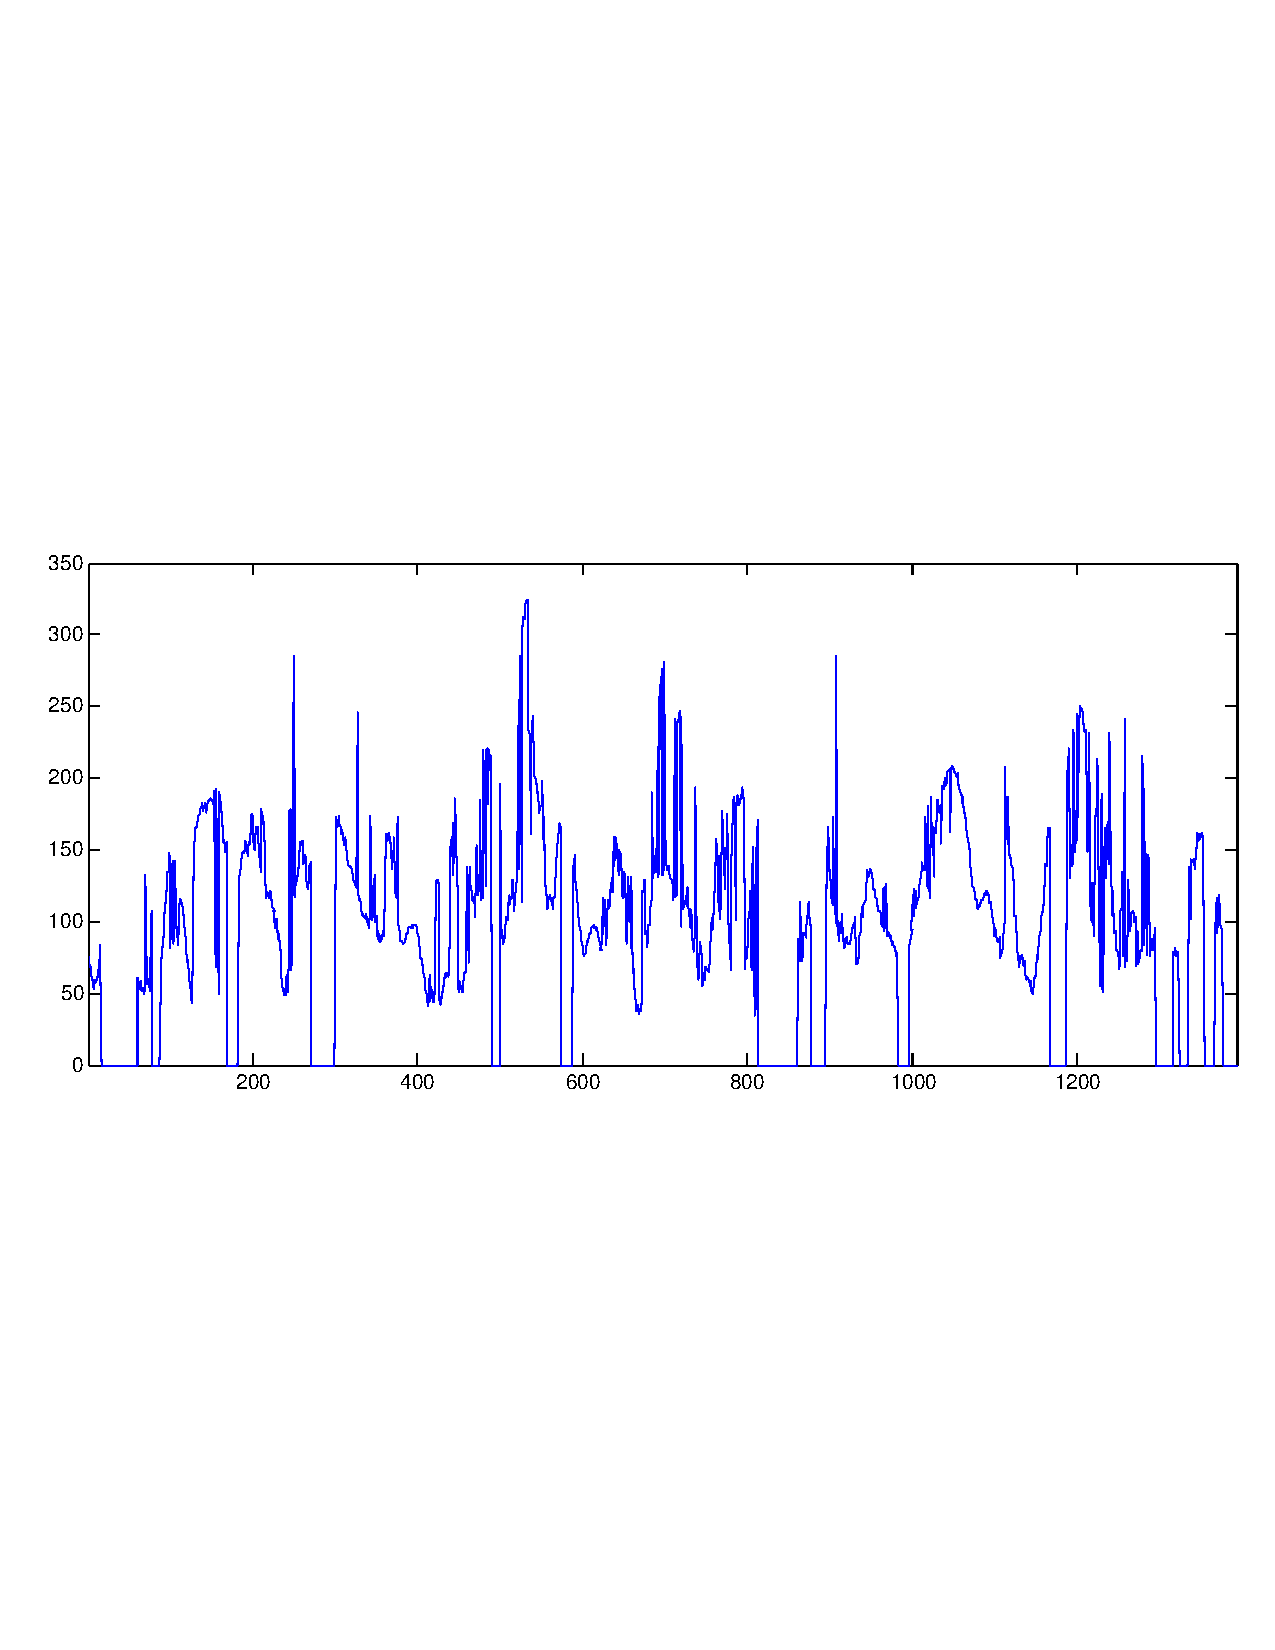
\includegraphics[width=0.7\textwidth]{S2_Throw}}\\
  \subcaptionbox{S4 Combo}{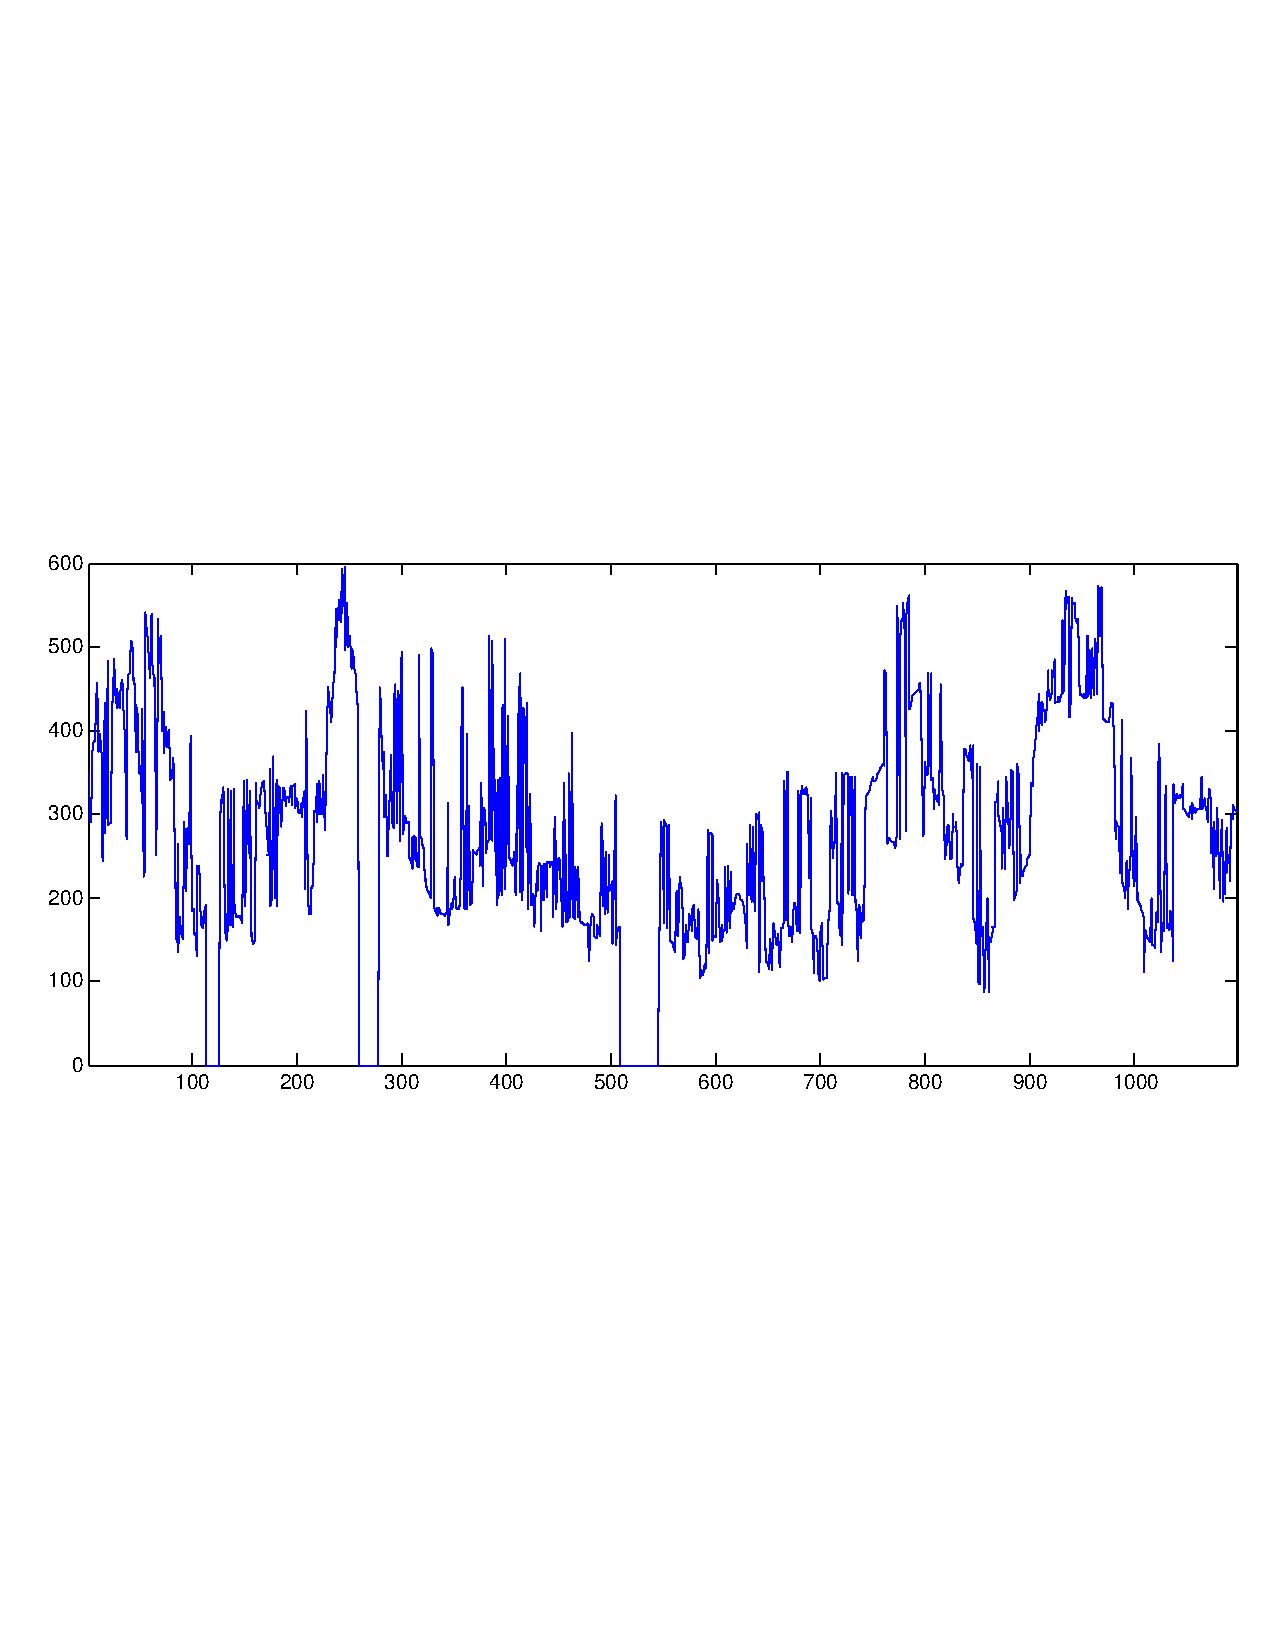
\includegraphics[width=0.7\textwidth]{S4_Combo}}
  \caption{单个视频逐帧误差}\label{fig:error}
\end{figure}

\subsection{其他数据}
本文将算法用于其他数据,发现无论是\cite{bo2010twin}的特征还是本文所提特征均表现不是很好,不过本文所提特征对于其他数据稍好一点。具体可以参考图\ref{fig:me},这是本人模仿数据库中动作所拍照片,对比结果见图,图\ref{fig:me_result}。可以看出本文结果更加接近真实情况,尤其是右臂部分。

\begin{figure}[htbp]
  \centering
  \subcaptionbox{C1}{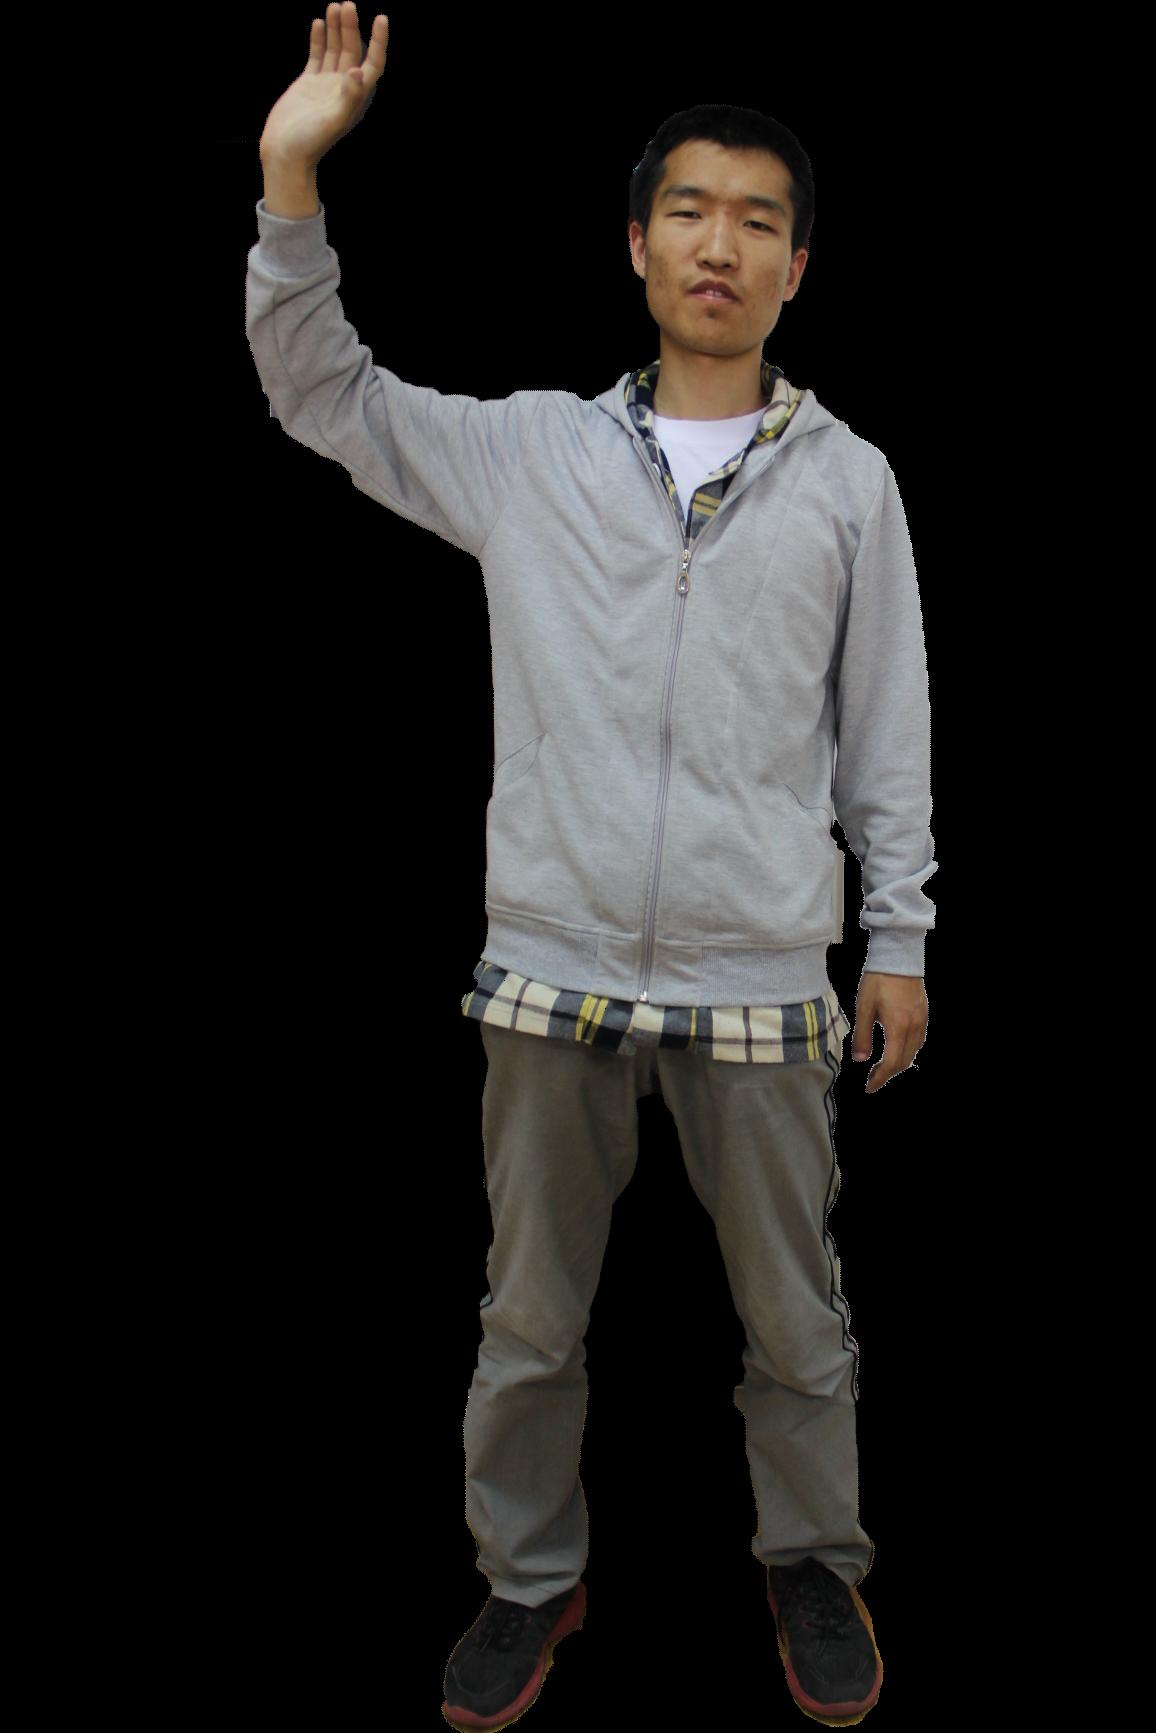
\includegraphics[width=0.2\textwidth]{me1}}\hspace{.5cm}
  \subcaptionbox{C2}{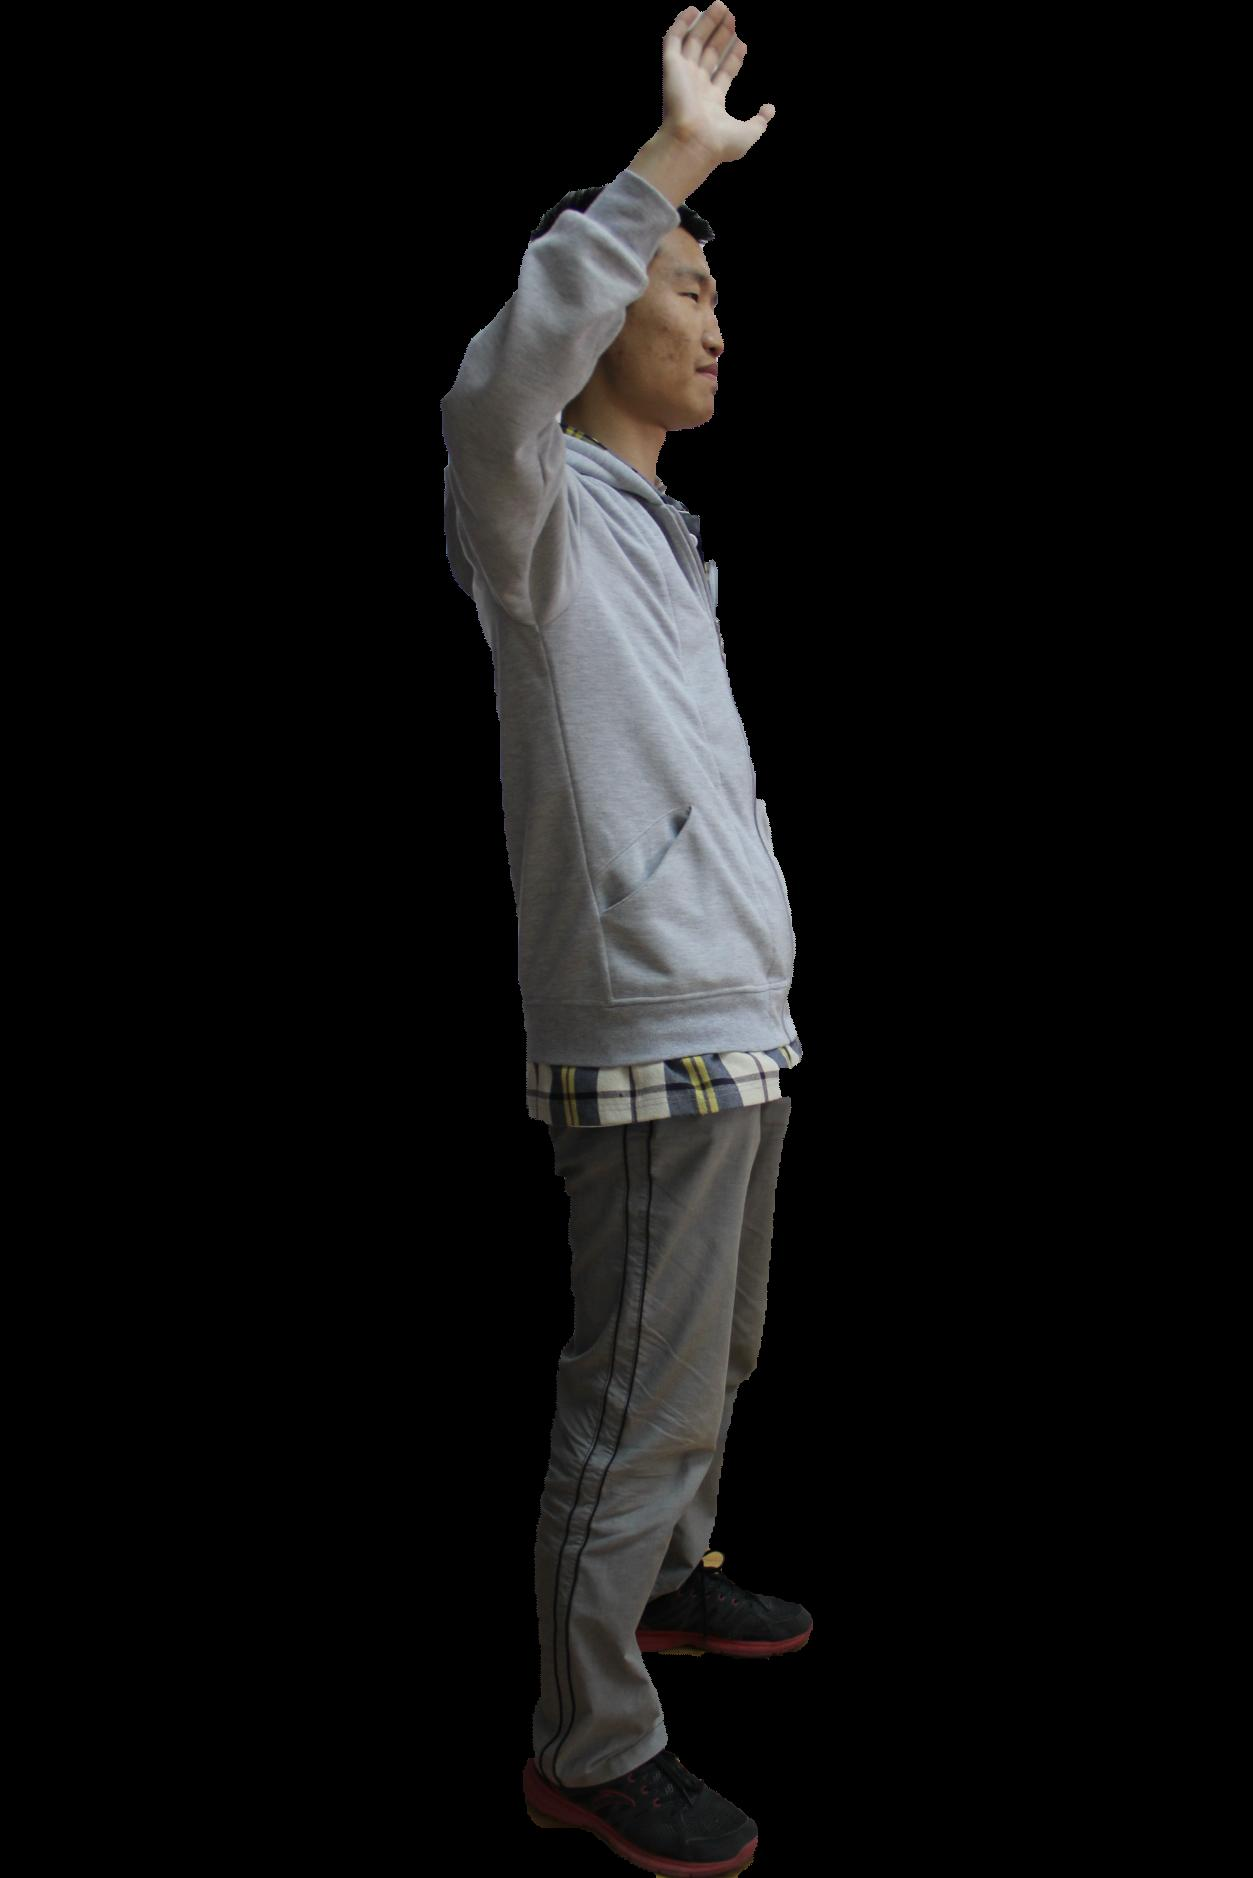
\includegraphics[width=0.2\textwidth]{me2}}\hspace{.5cm}
  \subcaptionbox{C3}{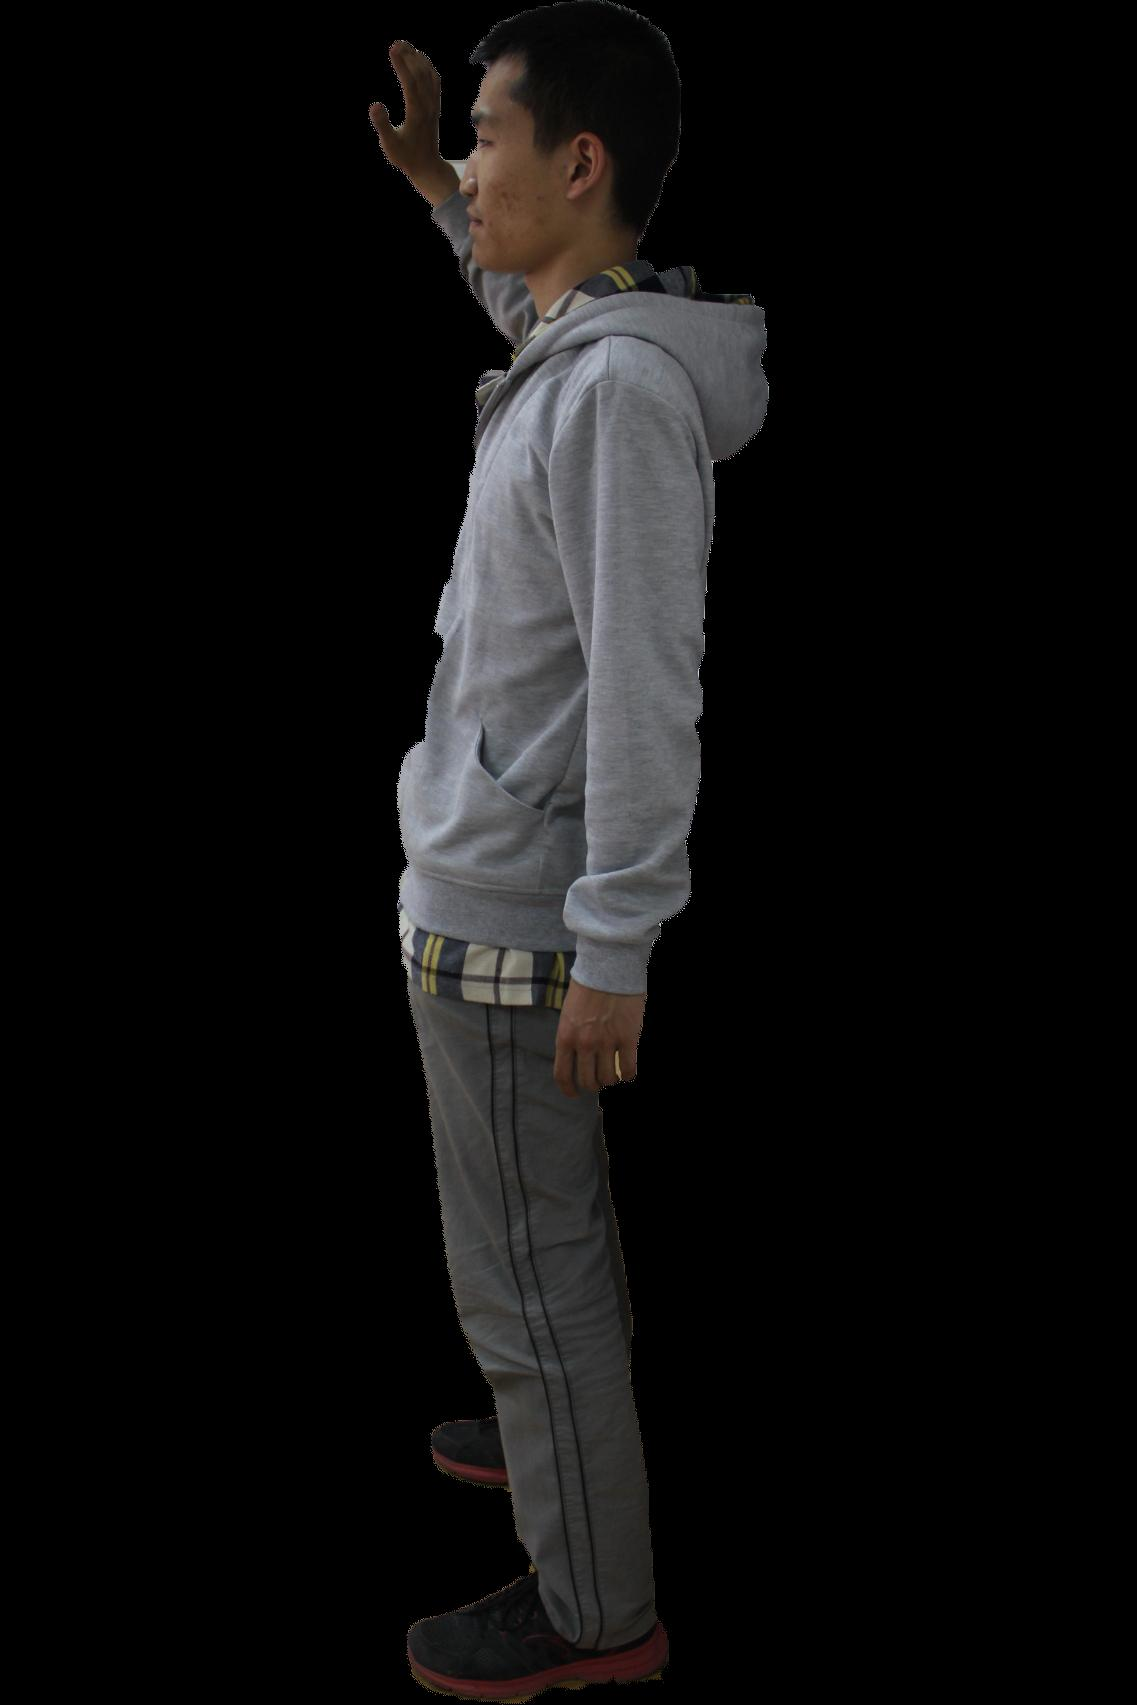
\includegraphics[width=0.2\textwidth]{me3}}\\
  \subcaptionbox{HOG1}{\includegraphics[width=0.2\textwidth]{meHOG1}}\hspace{.5cm}
  \subcaptionbox{HOG2}{\includegraphics[width=0.2\textwidth]{meHOG2}}\hspace{.5cm}
  \subcaptionbox{HOG3}{\includegraphics[width=0.2\textwidth]{meHOG3}}
  \caption{其他数据测试示意1}\label{fig:me}
\end{figure}

\begin{figure}[H]
  \centering
  \subcaptionbox{本文结果}{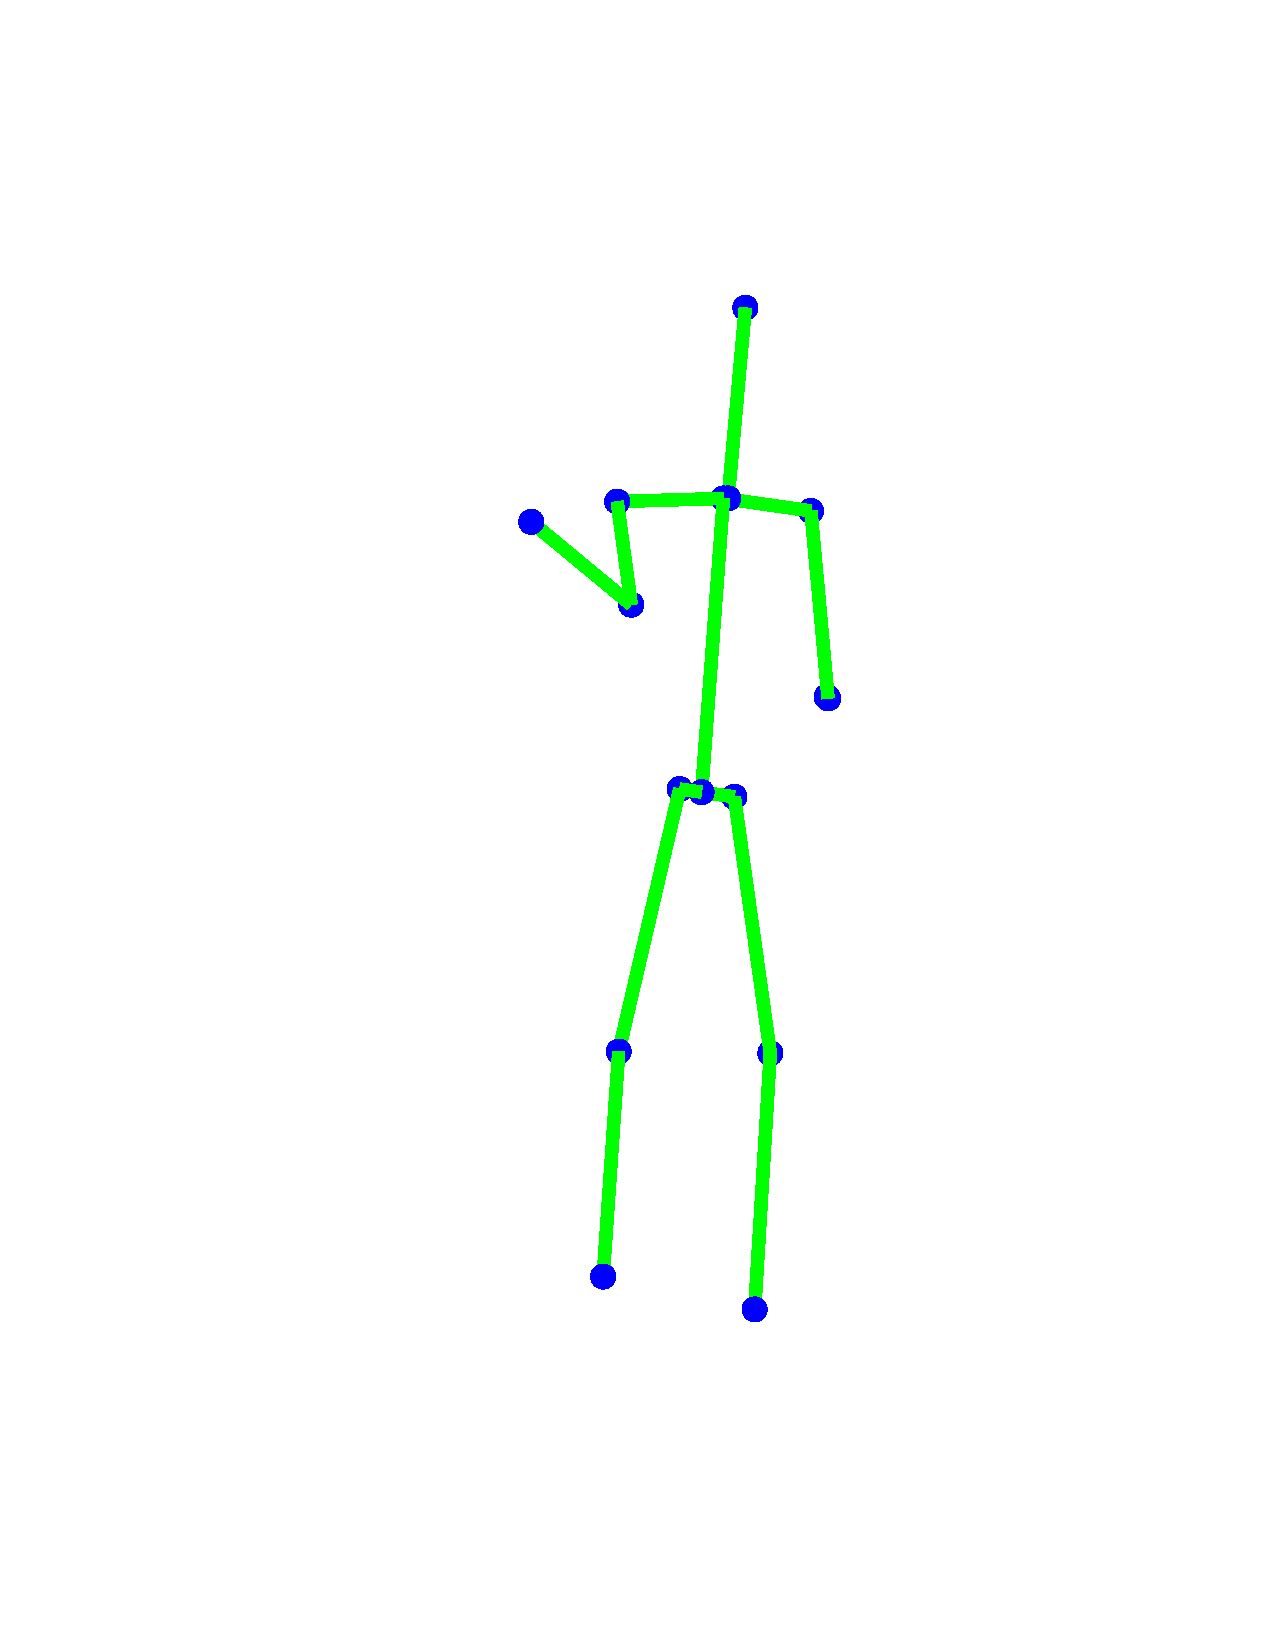
\includegraphics[height=5.5cm]{me_my}}\hspace{2cm}
  \subcaptionbox{\cite{bo2010twin}结果}{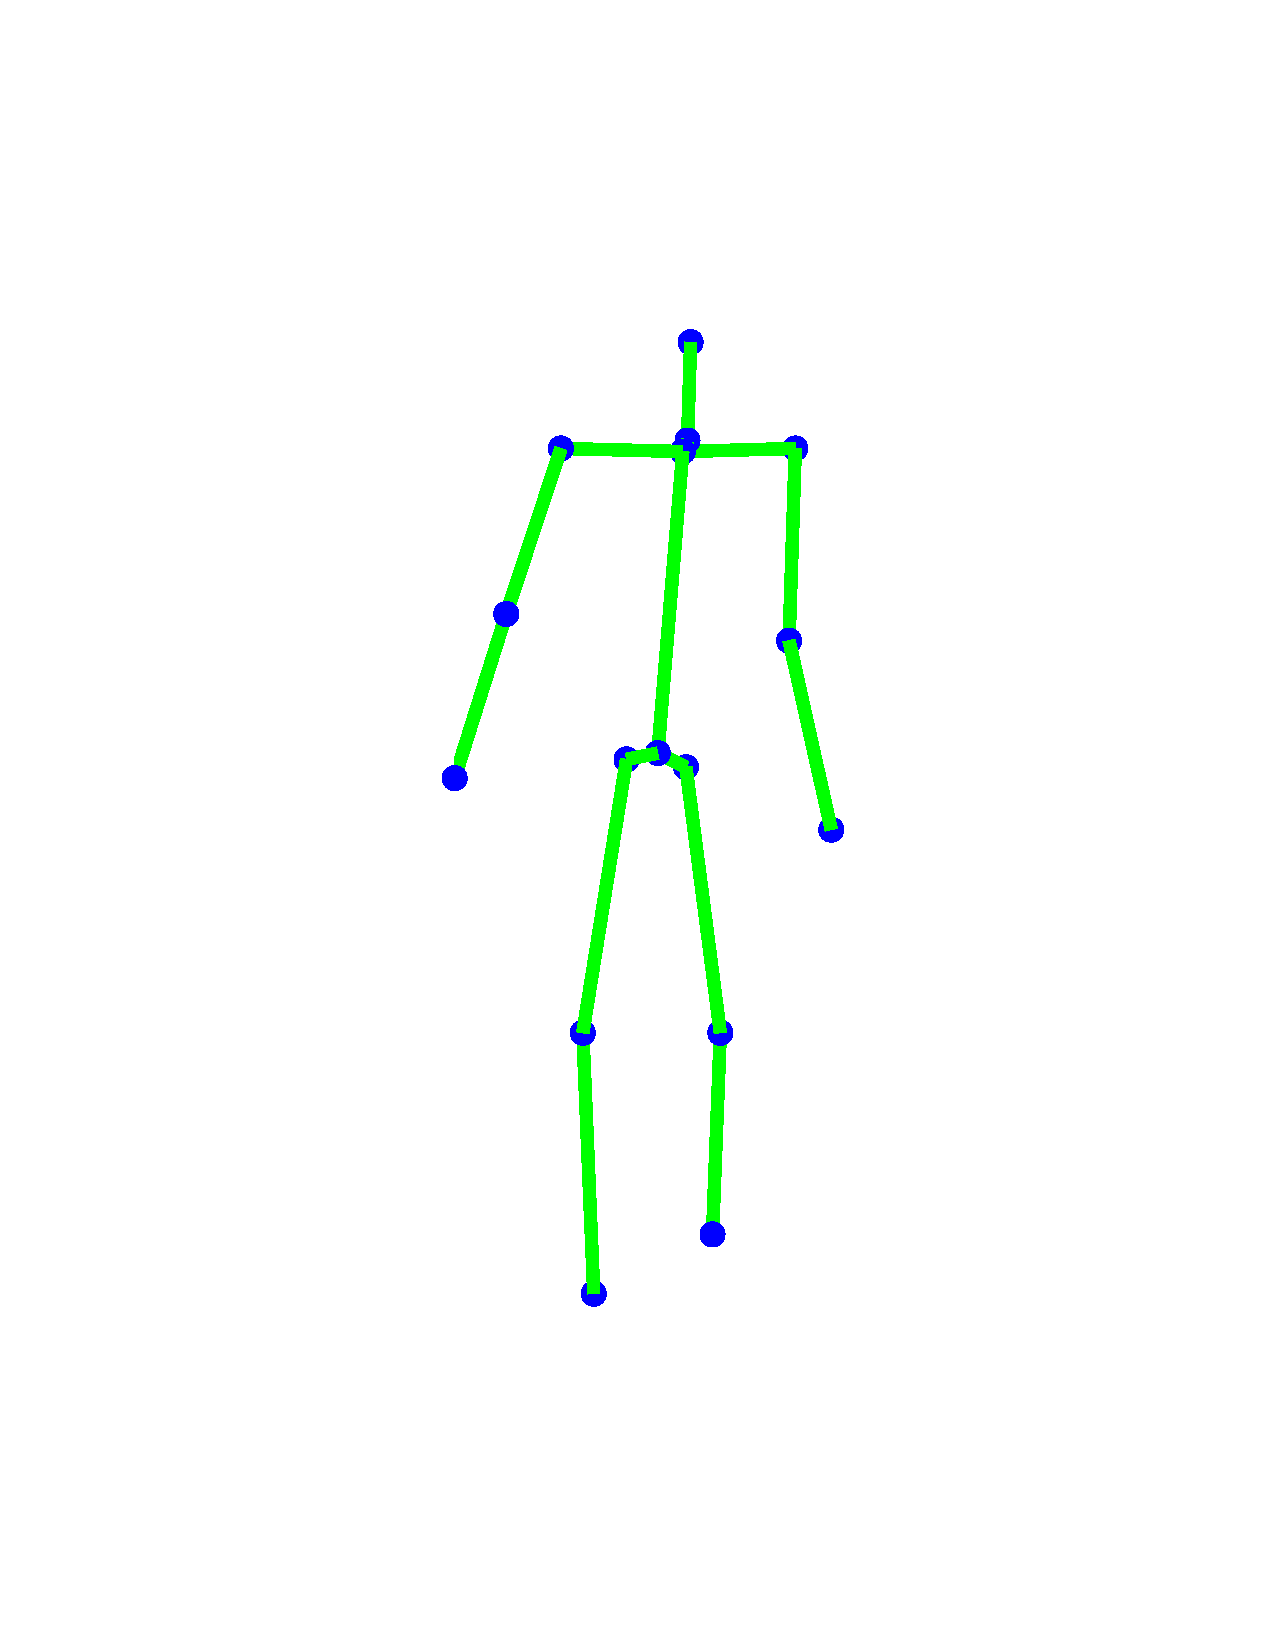
\includegraphics[height=5.5cm]{me_org}}
  \caption{其他数据测试结果对比1}\label{fig:me_result}
\end{figure}

图\ref{fig:mindance}是一位女性所做的简单动作,结果对比见图\ref{fig:mindance_result}。可以看出,两者结果差异不大,左臂都是错误的,但本文结果的右臂更加接近原图。

\begin{figure}[htbp]
  \centering
  \subcaptionbox{C1}{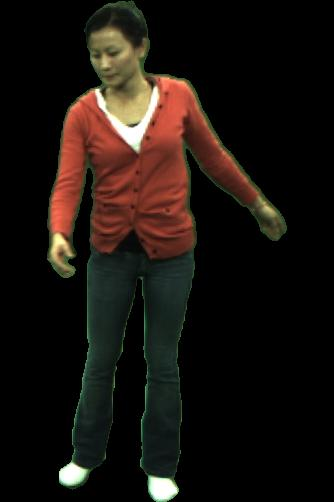
\includegraphics[width=0.2\textwidth]{mindance1}}\hspace{.5cm}
  \subcaptionbox{C2}{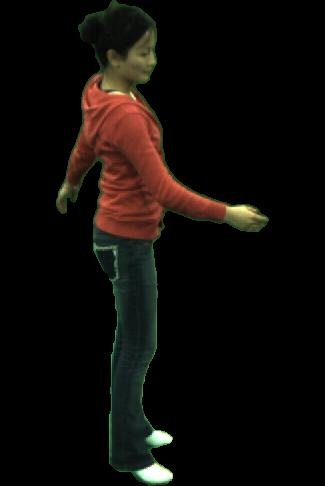
\includegraphics[width=0.2\textwidth]{mindance2}}\hspace{.5cm}
  \subcaptionbox{C3}{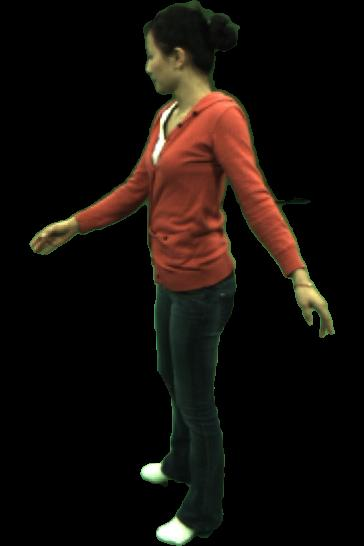
\includegraphics[width=0.2\textwidth]{mindance3}}\\
  \subcaptionbox{HOG1}{\includegraphics[width=0.2\textwidth]{mindanceHOG1}}\hspace{.5cm}
  \subcaptionbox{HOG2}{\includegraphics[width=0.2\textwidth]{mindanceHOG2}}\hspace{.5cm}
  \subcaptionbox{HOG3}{\includegraphics[width=0.2\textwidth]{mindanceHOG3}}
  \caption{其他数据测试示意2}\label{fig:mindance}
\end{figure}

\begin{figure}[H]
  \centering
  \subcaptionbox{本文结果}{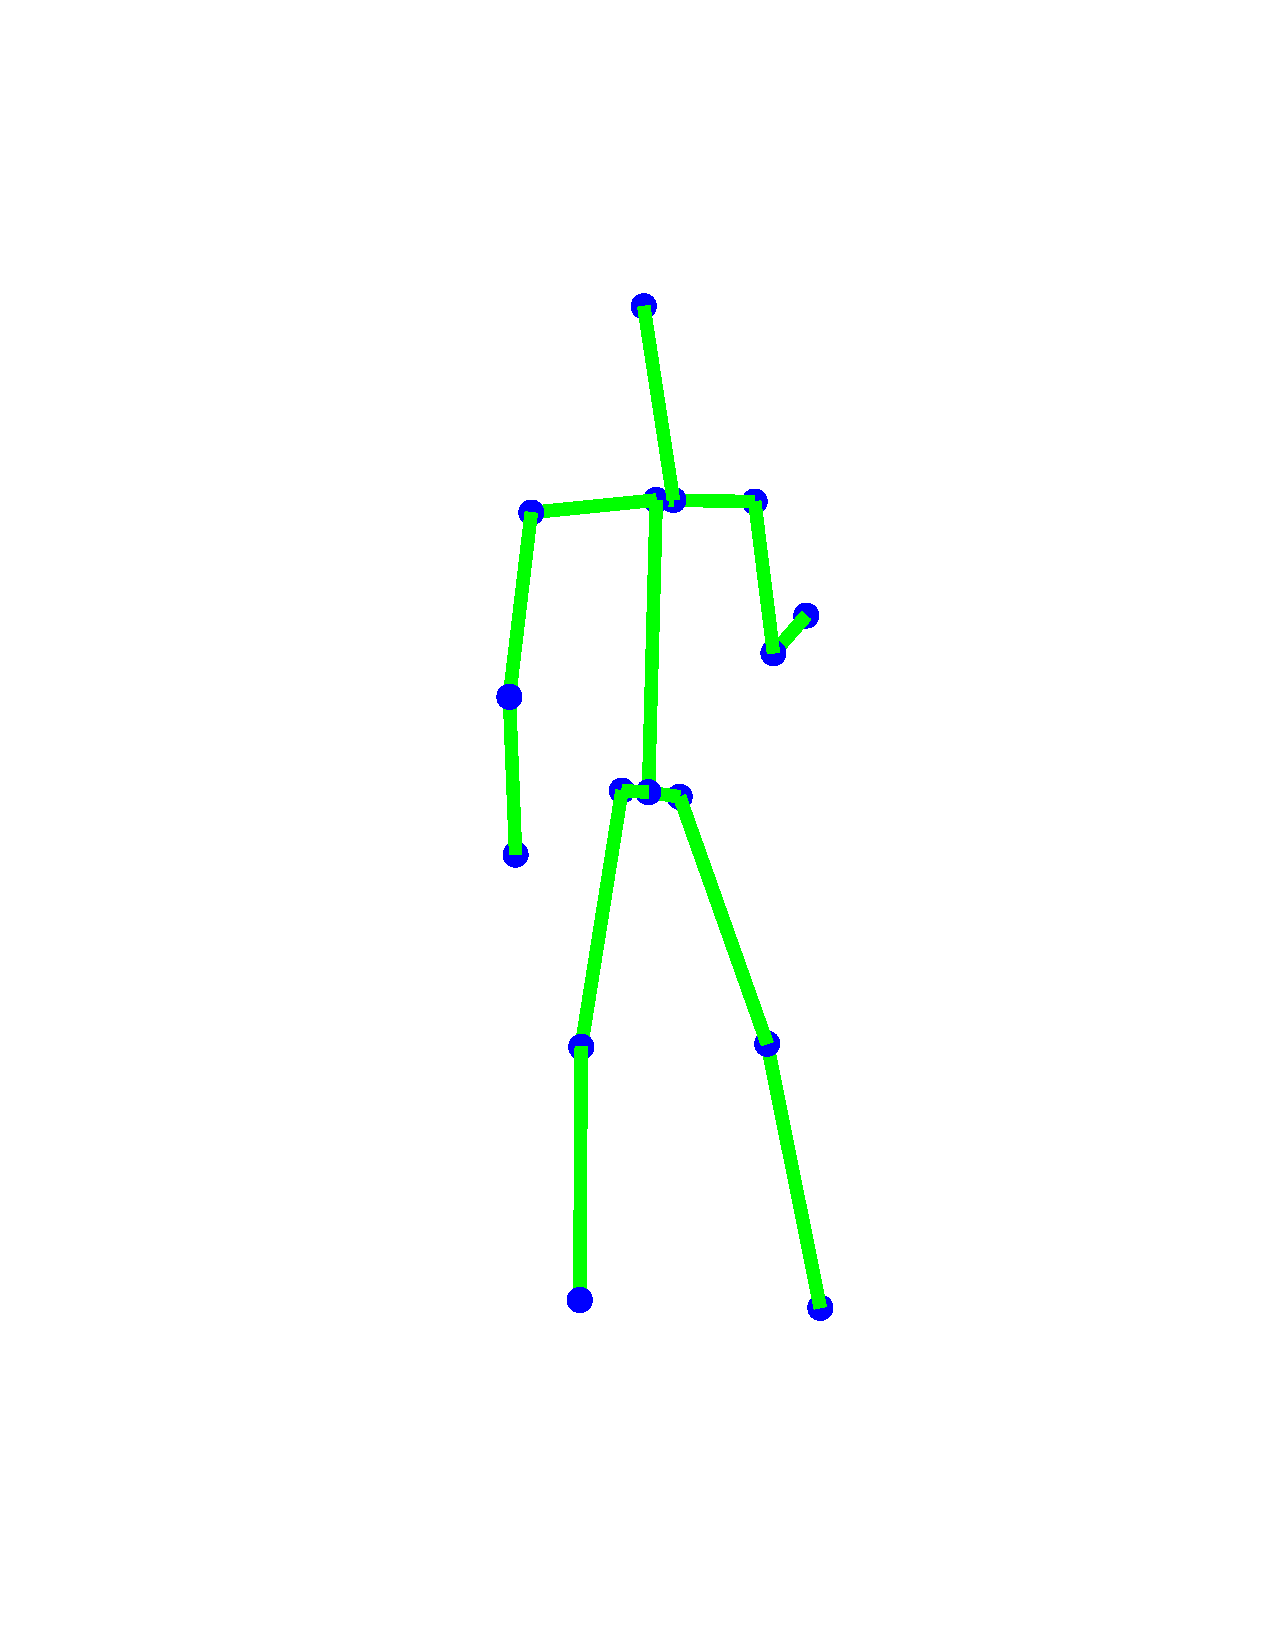
\includegraphics[height=5.5cm]{mindance_my}}\hspace{2cm}
  \subcaptionbox{\cite{bo2010twin}结果}{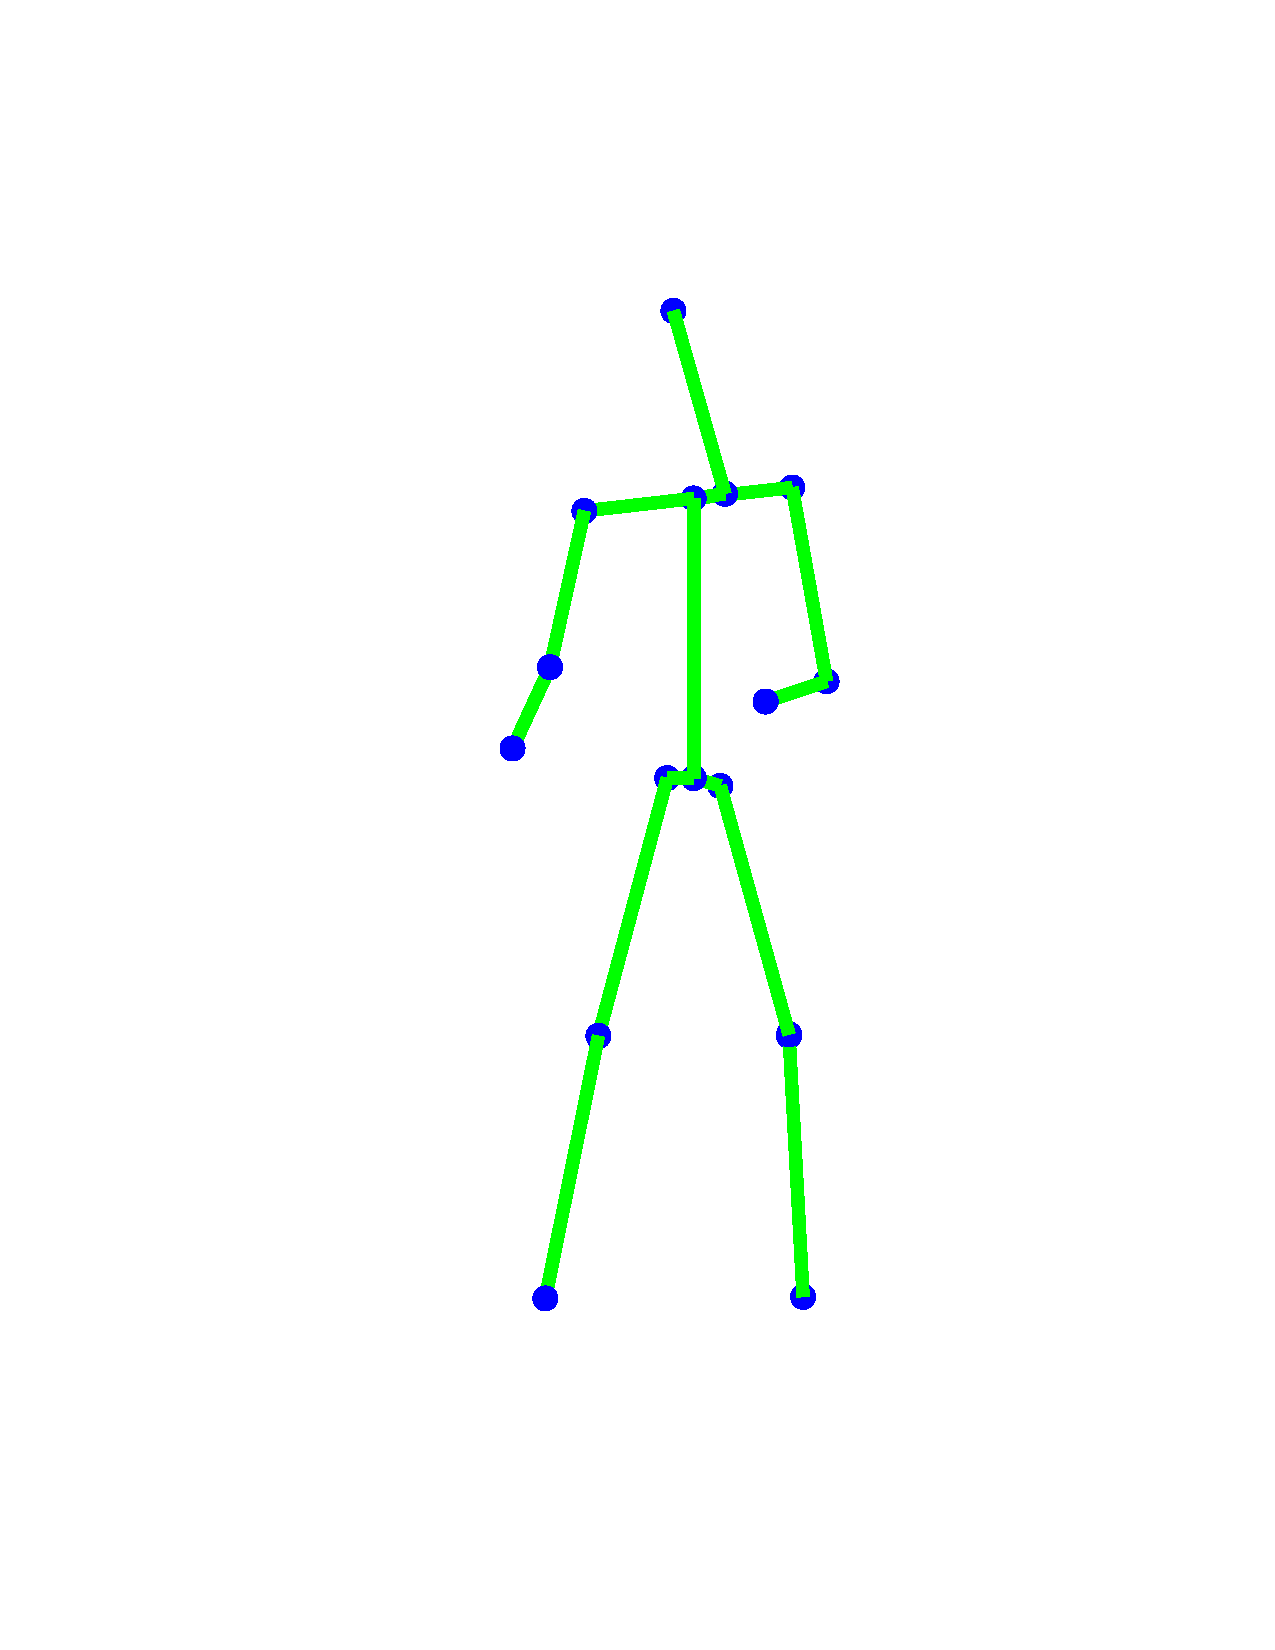
\includegraphics[height=5.5cm]{mindance_org}}
  \caption{其他数据测试结果对比2}\label{fig:mindance_result}
\end{figure}

\section{计算时间}
本文所做工作非常耗时,具体可以从表\ref{tab:time}看出。
\begin{table}[H]
  \centering
  \caption{测试各步骤耗时统计}
  \label{tab:time}
    \begin{tabular}{lccc}
      \toprule[1.5pt]
      步骤 & 帧数 & 耗时 & 单帧耗时\\\midrule[1pt]
      提取训练集特征 & 10232 & 9629 s $\approx$ 2.7 h & 0.94 s \\
      提取训练集ground-truth & 10232 & 1459 s $\approx$ 0.4 h & 0.14 s \\
      提取测试集特征 & 24000 & 22778 s $\approx$ 6.3 h & 0.95s\\
      训练TGP & - & 119 s & - \\
      预测测试集 & 24000 & 37781 s $\approx$ 10.5 h & 0.6 s\\
      网络测试 & 24000 & $\approx$ 12 h& 0.6 s\\
      \bottomrule[1.5pt]
    \end{tabular}
\end{table}

\section{结果分析}
\label{sec:analysis}
从以上结果可以看出本文所提特征在测试集上明显不如Bo等人~\cite{bo2010twin}的结果,可能的原因如下:
\begin{enumerate}
  \item 本文的背景分割方法在某些图片上效果不佳
  \item 本文所提HoG特征虽然没有改变图片比例,但改变了图片中人物的尺度
  \item 本文所用方法的参数选取不合适
\end{enumerate}

